\chapter{UML}
UML (\textbf{u}nified \textbf{m}odeling \textbf{l}anguage) è uno standard creato per unificare il modo di descrivere e progettare software in ambito della programmazione ad oggetti. 

\`E un linguaggio visuale che si basa su un meta-modello, un insieme di regole e vincoli per la modellazione di problemi software.
Ha una sintassi e una semantica ben definita. Uno dei vantaggi di UML è l'indipendenza dai linguaggi di programmazione.

I principali diagrammi trattati sono:
\begin{itemize}
\item diagrammi dei Casi d'Uso
\item diagrammi delle Classi
\item diagrammi dei Package
\item diagrammi di Sequenza
\item diagrammi di Attività
\end{itemize} 

\begin{figure}[H]
    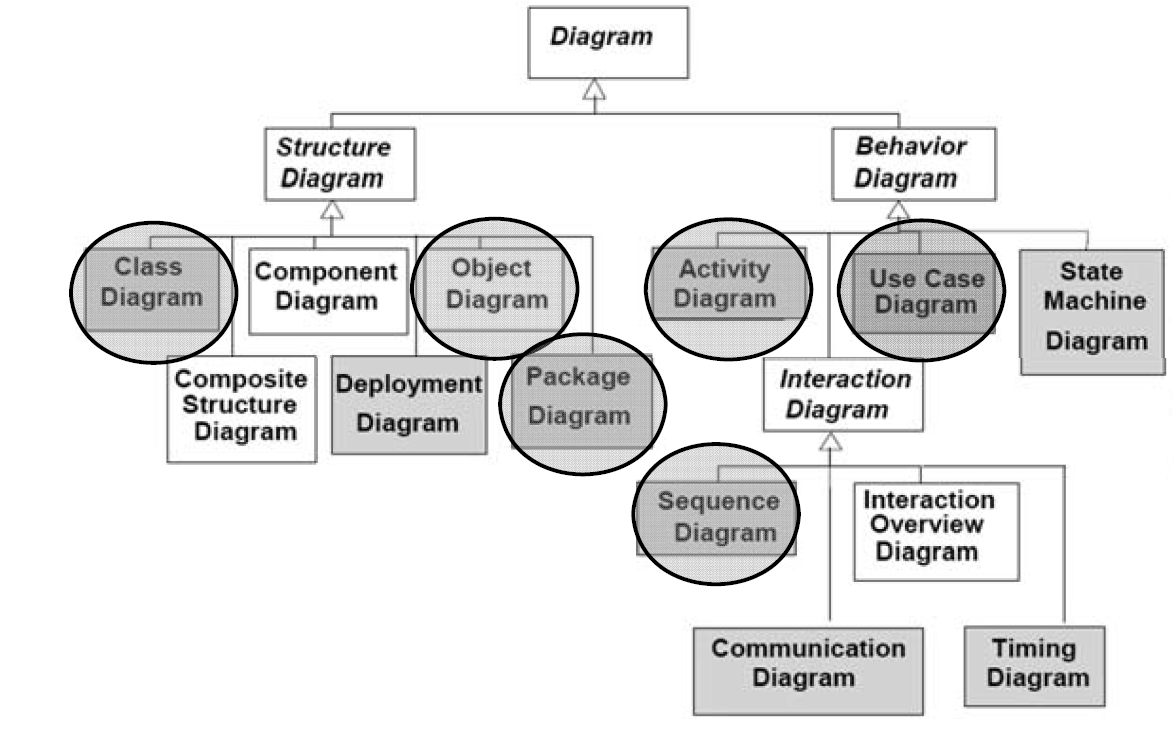
\includegraphics[width=1\textwidth]{res/img/diagrammiUML}
    \caption{Tipi di diagrammi in UML}
\end{figure}

\section{Diagrammi dei Casi d'Uso}

I diagrammi dei Casi d'Uso fanno parte dei diagrammi di comportamento. 

\subsection{I casi d'uso}
Un caso d'uso è un insieme di scenari (sequenze di azioni) che hanno in comune uno scopo finale (obiettivo) per un utente (attore),
\textit{cioè} un caso d'uso è una situazione nella quale il sistema viene utilizzato per soddisfare uno o più bisogno dell'utente.

Le funzionalità vengono descritte secondo la visione esterna, ovvero come vengono viste dall'utente, e non hanno nessun dettaglio implementativo.

I casi d'uso sono descrizioni puramente testuali, mentre i diagrammi dei casi d'uso vengono descritti con UML e rappresentano graficamente le relazioni tra attori e casi d'uso.

Un caso d'uso deve essere elementare, cioè non scomponibile in casi d'uso più semplici che abbiano ancora senso compiuto per gli attori coinvolti. 
Deve essere più grande di una singola operazione su un componente. 

Elementi di un caso d'uso:
\begin{itemize}
\item Nome + Identificatore - il nome deve essere più chiaro possibile;
\item Attori principali;
\item Attori secondari;
\item Pre-condizioni;
\item Post-condizioni; 
\item Scenario principale - la sequenza di azioni svolte dagli attori e dal sistema;
\item Scenari alternativi - eccezioni/errori e come devono essere gestiti;
\item Trigger - evento scatenante del caso d'uso.
\end{itemize}

\subsubsection{Attori}

Un attore è colui che svolge il caso d'uso per raggiungere un certo obiettivo. Può essere una persona o un altro sistema. 

Un utente può avere più ruoli (diversi attori); più utenti possono avere il medesimo ruolo (singolo attore). 

Un attore può essere collegato a più casi d'uso e un caso d'uso può avere più attori. \\
Come identificare un attore:
\begin{enumerate}
\item Identificare un entità
\item L'entità è una persona che interagisce con il sistema?
\begin{itemize}
\item[\texttt{SI}] $\to$ potrebbe essere un attore, ma si deve fare attenzione alle persone che potrebbero comunque essere parte del sistema.
\item[\texttt{NO}] $\to$ l'entità è qualcosa che si può cambiare all'interno del design del sistema?
\begin{itemize}
\item[\texttt{NO}] $\to$ probabilmente è un attore.
\item[\texttt{SI}] $\to$ l'entità non dovrebbe essere un attore, in quanto tutto ciò su cui è possibile avere il controllo, è da considerarsi parte del sistema.
\end{itemize}
\end{itemize}
\end{enumerate}

\subsection{I diagrammi}

I diagrammi dei casi d'uso sono grafi con gli attori e i casi d'uso come nodi, mentre gli archi rappresentano la comunicazione attore-caso d'uso e le relazioni tra casi d'uso, che possono essere:
\begin{itemize}
\item inclusione
\item estensione
\item generalizzazione
\end{itemize}

\begin{figure}[H]
    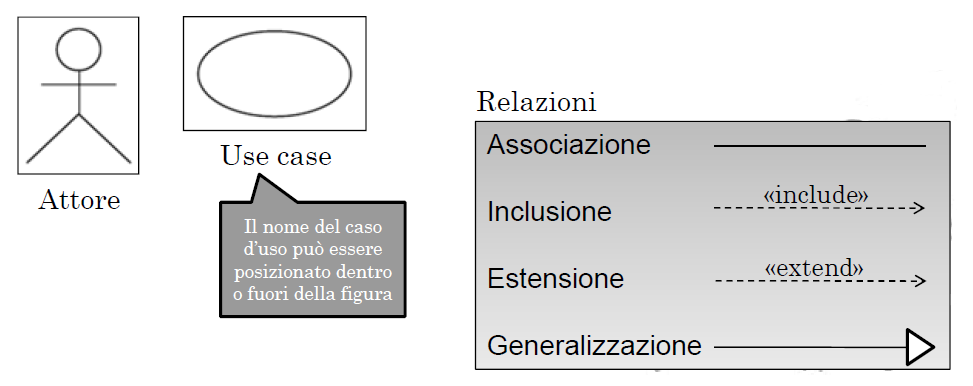
\includegraphics[width=1\textwidth]{res/img/componentiUseCaseDiagram}
    \caption{Componenti diagrammi dei Casi d'Uso (\textit{Slide E02})}
\end{figure}

\subsubsection{Inclusione}
L'inclusione viene utilizzata quando una funzionalità è comune a più casi d'uso. 
\texttt{A <<include>> B} indica che ogni istanza di A esegue B in modo incondizionato. 
A non conosce i dettagli di B, ma solo i risultati. Allo stesso modo, B non sa di essere incluso in A.

\subsubsection{Estensione}
L'estensione aumenta le funzionalità di un caso d'uso. 
\texttt{A <<extend>> B} indica che ogni istanza di A esegue B in modo condizionato, cioè l'esecuzione di B interrompe A.
Questa relazione viene spesso utilizzata per isolare in uno caso d'uso a parte la specifica di attività opzionali 
o eccezionali che potrebbero aver luogo durante l'esecuzione della funzione principale.

\subsubsection{Inclusione vs Estensione}
Entrambe le relazioni aumentano il comportamento di un caso d'uso e possono essere comuni a più casi d'uso. 
Nell'inclusione, un attore esegue sempre tutte le inclusioni, mentre nell'estensione l'attore può non eseguirle tutte.
Quindi, un'inclusione viene usata se una funzionalità si ripete in più casi d'uso; 
l'estensione se si vogliono descrivere variazioni dalla funzionalità standard. 

\subsubsection{Generalizzazione}
La generalizzazione aggiunge o modifica delle caratteristiche di base. 
Può essere usato tra attori o tra casi d'uso (più raro). 
A è generalizzazione di B se B condivide almeno le funzionalità di A.

\subsection{Individuazione Casi d'Uso}

Definizione del contesto:
\begin{enumerate}
\item Identificazione attori e responsabilità
\item Identificazione degli obiettivi da raggiungere per ciascun attore
\item Valutare attori e casi d'uso e raffinarli (divisione e accorpamento)
\item Trovare le relazioni di inclusione
\item Trovare le relazioni di estensione
\item Trovare le relazioni di generalizzazione
\end{enumerate}
Livello di dettaglio:
\begin{itemize}
\item \textbf{Kite level} - Livello molto astratto, definisce macro funzionalità
\item \textbf{Sea level} - Livello intermedio, utile nella scoperta di funzionalità nascoste
\item \textbf{Fish level} - Livello di dettaglio, da esso si individuano direttamente i requisiti del sistema
\end{itemize}

\section{Diagrammi delle Classi}
I diagrammi delle classi fanno parte dei diagrammi di struttura e si usano per rappresentare i tipi di oggetti che fanno parte di un sistema e le relazioni statiche fra i tipi. 

\subsection{Le classi}
Una classe si rappresenta:
\begin{table}[H]
\centering
\begin{tabular}{|l|}
\hline
\textbf{Nome della classe} \\
\hline
Attributo 1 \\
... \\
Attributo N \\
\hline
Operazione 1 \\
... \\
Operazione M \\
\hline
\end{tabular}
\caption{Rappresentazione di un classe}
\end{table}
Solo il nome della classe è obbligatorio, il resto è opzionale. \\
Un \textbf{attributo} è definito con:
\begin{verbatim}
Visibilità nome : tipo [molteplicità] = default {proprietà aggiuntive}
\end{verbatim}
La visibilità può essere:
\begin{itemize}
\item[\texttt{+}] public
\item[\texttt{\#}] protected
\item[\texttt{\textasciitilde}] package
\item[\texttt{-}] private
\end{itemize}
Un'\textbf{operazione} è un'azione che la classe sa eseguire ed è un servizio che può esser richiesto da ogni oggetto. Si definisce con:
\begin{verbatim}
Visibilità nome (lista-parametri) : tipo-ritorno {proprietà aggiuntive}

lista-parametri := direzione nome : tipo = default
\end{verbatim}
La visibilità si indica come per gli attributi, mentre la direzione può essere:
\begin{itemize}
\item in (default)
\item out
\item inout
\end{itemize}
Un'operazione è detta \textit{modificatore} se modifica lo stato dell'oggetto; è detta \textit{query} se non modifica lo stato. \\
\textbf{NB}: Non c'è una relazione diretta tra operazione e metodo.

Di solito i membri di una classe si indicano in: % non sono 100% sicuro che sia uno standard UML
\begin{itemize}
\item \underline{sottolineato} se è statico
\item \textit{corsivo} se è astratto
\item MAIUSCOLO se è costante
\end{itemize}

\`E possibile aggiungere \textbf{commenti} e note in un riquadro, collegandolo con una linea tratteggiata al punto di interesse.

\subsection{Relazioni tra classi}

Due classi possono essere collegate da diversi tipi di relazione, ognuna rappresentata da un diverso tipo di freccia:
\begin{itemize}
\item dipendenza
\item associazione
\item aggregazione
\item composizione
\item generalizzazione
\end{itemize}

\begin{figure}[H]
    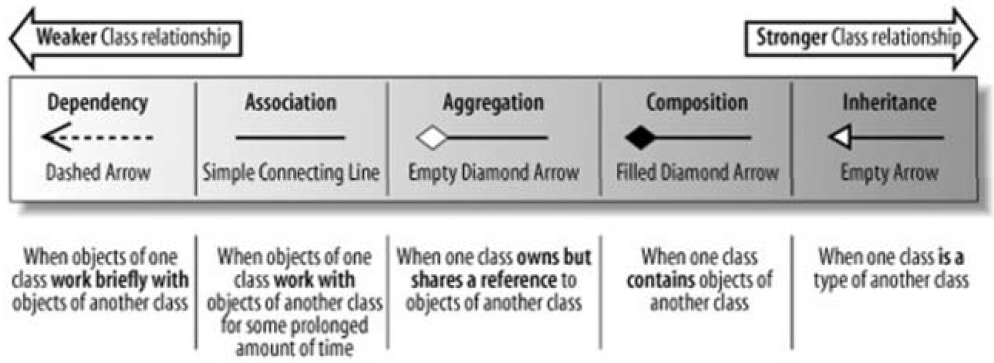
\includegraphics[width=1\textwidth]{res/img/relazioniClassi}
    \caption{Relazioni tra classi (\textit{Slide E03})}
\end{figure}

\subsubsection{Dipendenza}
Si ha una relazione di dipendenza se la modifica della definizione di un elemento può cambiare la definizione del secondo elemento. 
Maggiore è il codice condiviso tra due classi, maggiore è la dipendenza. Le dipendenze sono da minimizzare.

\textit{[Manca la lista di dipendenze UML]}

\subsubsection{Associazione}
Un'associazione rappresenta una connessione logica tra due classi ed è descritta da una linea che collega due classi 
(può essere orientata se ha senso in un solo verso); a volte ha un'etichetta ed è preferibile che sia un nome piuttosto che un verbo.

Ogni associazione può avere la molteplicità che indica il numero di istanze di una classe che possono essere associate ad una singola istanza dell'altra classe (1, 0..1, 0..*, *).

\`E possibile usare classi di associazione che aggiungono attributi e operazioni alle associazioni e non direttamente alle classi. 
\`E una sorta di classe intermedia; per ogni coppia di oggetti, esiste \textbf{una sola} istanza della classe associazione. 

La classe di associazione è collegata all'associazione con una linea tratteggiata e si può leggere come "è un insieme di".

\subsubsection{Aggregazione}
Indica una relazione "parte di". Gli aggregati possono essere condivisi. Il \textit{diamante vuoto} della freccia è il punto di partenza della relazione.

\subsubsection{Composizione}
Come nell'aggregazione, indica una relazione "parte di", ma gli aggregati appartengono ad un solo oggetto e quest'ultimo è l'unico che può creare o distruggere le sue parti. 

Il \textit{diamante pieno} della freccia è il punto di partenza della relazione e si può leggere come "è composto da".

\subsubsection{Generalizzazione}
La generalizzazione equivale all'ereditarietà nei linguaggi di programmazione. 
A generalizza B se ogni oggetto di B è anche oggetto di A. Le proprietà ereditate non vanno ripetute nella sottoclasse.

Esistono anche la classi astratte e le interfacce. Le classi astratte hanno il nome in corsivo o \texttt{nome \{abstract\}}. La classe non è istanziabile e alcune delle operazioni non hanno implementazioni. 

Le interfacce sono classi prive di implementazioni e si indicano con \texttt{<<interface>> nome} nella solita forma tabellare (UML 1) o si usa un pallino con sotto il nome e le operazioni (UML 2). 
In entrambi i casi viene collegata alla classe che implementa l'interfaccia.

\subsection{Diagrammi degli oggetti}
\`E un grafo delle singole istanze, comprensivo di associazioni e valori delle proprietà.

\begin{table}[H]
\centering
\begin{tabular}{|l|}
\hline
nome dell'istanza : nome della classe \\
\hline
nome dell'attributo = valore \\
\hline
\end{tabular}
\caption{Diagramma di un oggetto}
\end{table}

\section{Diagrammi dei Package}
I diagrammi dei package fanno parte dei diagrammi di struttura. 

\subsection{I package}
Un package è un raggruppamento di elementi UML (di solito classi) usato per creare un namespace.
Un package può contenere più package, creando una struttura gerarchica.

Ogni elemento deve avere un nome distinto e il nome completo è identificato da:
\begin{verbatim}
package::package::…::classe
\end{verbatim}
Gli elementi del package possono avere visibilità pubblica (+) o privata (-). \\
Ci sono due modi di progettare i package:
\begin{itemize}
\item \textbf{Common Closure Principle} - le classi dello stesso package condividono la stessa causa di cambiamento;
\item \textbf{Common Reuse Principle} - le classi dello stesso package dovrebbero essere sempre riusate insieme.
\end{itemize}
L'interfaccia di un package è l'insieme dei tipi pubblici del package.
Un package è invece detto \textit{di interfaccia} se contiene interfacce e classi astratte. 


\subsection{I diagrammi}

I diagrammi dei package sono utili per documentare le dipendenze tra le classi. 
Le dipendenze dovrebbero essere tutte dello stesso verso e si devono evitare le dipendenze circolari. 
Più dipenenze entranti ha package, più il package stesso dovrebbe essere stabile.

\section{Diagrammi di Sequenza}
I diagrammi di sequenza fanno parte dei diagrammi di comportamento e servono per descrivere come un gruppo di oggetti implementano un comportamento.

 



\section{Diagrammi di Attività}
I diagrammi di attività fanno parte dei diagrammi di comportamento e si utilizzano per descrivere gli aspetti dinamici dei casi d'uso. 
